\chapter{L’échantillonnage}
On détermine parfois un signal continu $x(n)$ par des échantillons prélevée à période $T$, 
$x(nT)$. Nous allons ici considérer des gianux à TC (on utilisera $\Omega$ en rad/s) et 
TD ($\omega$ en rad).

	\section{Échantillonnage par un train d'impulsions}
	\begin{wrapfigure}[12]{l}{4.5cm}
	\vspace{-5mm}
	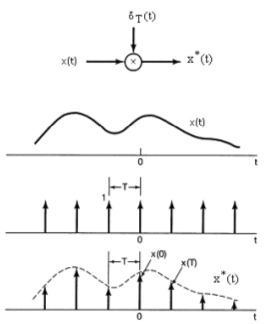
\includegraphics[scale=0.45]{ch4/image1.png}
	\captionof{figure}{ }
	\end{wrapfigure}
	L'idée est de moduler $x(t)$ avec un train périodique d'impulsion de Dirac. On obtient 
	ainsi le signal impulsionnel $x^*(t)$ 
	\begin{equation}
	x^*(t) = x(t)\delta_T(t) = x(t)\sum_{n=-\infty}^\infty \delta(t-nT)
	\end{equation}
	Il s'agit bien d'une multiplication et non d'une convolution.  On appelle $T$ la 
	\textit{période d’échantillonnage}, $\Omega_S = 2\pi/T$ la \textit{pulsation d’échantillonnage} 
	et $f_S=1/T$ la \textit{fréquence d’échantillonnage}.\\
	
	Comme $\delta_T(t)$ est périodique, on peut utiliser la série de Fourier (calculée à la fin 
	du chapitre précédent)
	\begin{equation}
	\begin{array}{ll}
	\delta_T &=\DS \sum_{n=-\infty}^\infty \delta(t-nT)\\
	&= \DS \dfrac{1}{T}\sum_{n=-\infty}^\infty e^{jk\frac{2\pi}{T}t}
	\end{array}
	\end{equation}
	Il s'agit d'une série infinie d'exponentielles complexes. En substituant dans l'équation
	\begin{equation}
	x^*(t) = \frac{1}{T}x(t)\sum_{k=-\infty}^\infty e^{jk\Omega_St}
	\end{equation}
	Calculons-en sa transformée de Laplace (premier pas vers la transformée de Fourier)
	\begin{equation}
	X^*(p) = \mathcal{L}[x^*(t)] = \dfrac{1}{T}\sum_{k=-\infty}^\infty \mathcal{L}\left[x(t)
	e^{jk\Omega_St}\right]
	\end{equation}
	En posant $\alpha = jk\Omega_S$ on retrouve une forme équivalente à un décalage dans le temps
	\begin{equation}
	\int_{-\infty}^\infty \left(x(t)e^{\alpha t}\right)e^{-pt}\ dt = \int_{-\infty}^\infty x(t) 
	e^{-(p-\alpha)t}\ dt = X(p-\alpha)
	\end{equation}
	La transformée de Laplace de la multiplication par une exponentielle imaginaire donne un 
	décalage dans le temps (soit notre expression en substituant $\alpha$
	\begin{equation}
	x(t)e^{jk\Omega_st}\qquad \lt\qquad \frac{1}{T}\sum_{k=-\infty}^\infty X(p-jk\Omega_S)
	\end{equation}
	En particularisant pour $p = j\Omega$, on trouve
	\begin{equation}
	X^*(\Omega) = \dfrac{1}{T}\sum_{k=-\infty}^\infty X(\Omega-k\Omega_S)
	\end{equation}
	On retrouve dans la série le spectre du signal en entrée : on a copié/collé une infinité 
	de fois le spectre décalé vers la gauche et la droite. Un signal échantillonné dans le temporel 
	présente donc un spectre périodique de période $\Omega_S$.
	\begin{wrapfigure}[10]{l}{8.5cm}
	\vspace{-5mm}
	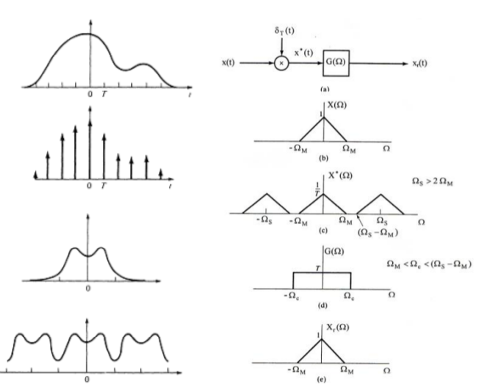
\includegraphics[scale=0.5]{ch4/image2.png}
	\captionof{figure}{ }
	\label{fig:rec}
	\end{wrapfigure}	
	Cependant, les spectres décalés vont se recouvrir : on ne pourra plus avoir $X$ à partir 
	de $X^*$. Si $\exists \Omega_M : X(\Omega) = 0$ pour $|\Omega|>\Omega_M$, alors il n'y aura 
	pas de recouvrement si la fréquence d’échantillonnage est assez grande : $\Omega_S > 2\Omega_M$.\\
	
	Si cette condition est satisfaite, on pourra reconstituer $x(t)$ à partir du signal 
	échantillonné $x^*(t)$ dans un filtre passe-bas idéal $G(\Omega)$ de gain $T$ et de 
	fréquence de coupure $\Omega_c$ tel que
	\begin{equation}
	\Omega_M < \Omega_c < \Omega_S-\Omega_M
	\end{equation}
	C'est le théorème de Shannon :\\
	\theor{\ \textsc{Shannon}\\
	La fréquence d'échantillonage doit être supérieure au double de la fréquence maximale 
	du signal. Celui-ci est alors entièrement caractérisé}\ \\
	\vspace{2cm}
	\exemple{Si l'on fait tourner une foreuse plus rapidement que le taux d’échantillonnage, 
	Shannon n'est pas respecté : on perd en information. Pire, on pense que la foreuse est 
	"à l'arrêt" alors qu'il n'en est rien.\\
	
	\textbf{
	Petit plus pour comprendre}\footnote{Source : Wikipedia} : "\textit{Cette distorsion se produit parce qu'un signal de fréquence fréquence porteuse $- f$ a exactement le même effet sur le signal modulé que ceux de fréquence $f$. De même, dans le cas d'un signal échantillonné, tous les signaux dont l'écart de fréquence avec la fréquence d'échantillonnage est identique se représentent par les mêmes échantillons. Lorsqu'on reconstitue le signal d'origine, il est impossible de distinguer ces composantes dont la représentation est identique.}.}\ \\
	\vspace{3mm}
	
	Sur la \autoref{fig:rec} : à gauche, on voit que la fonction périodique implique un recouvrement. A 
	droite on effectue une convolution dans le temporel. Un filtre idéal coupe à $\Omega_c$ (quand 
	le spectre s'est arrêté et avant qu'il ne reprenne). On n'a alors pas perdu d'information (retour 
	exact au signal initial).
	
	\newpage
	\section{Formule d'interpolation}
	Appliquons la convolution  pour retrouver notre signal de base
	\begin{equation}
	x(t) = x^*(t)*g(t) = \int_{-\infty}^\infty x^*(\tau)g(t-\tau)\ d\tau
	\end{equation}
	où $g(t) = \frac{T}{\pi t}\sin\Omega_ct$, un filtre passe-bas idéal de gain $T$ et de fréquence 
	de coupure $\Omega_c$. On peut prendre $\Omega_c = \frac{\Omega_S}{2}=\frac{\pi}{T}$ : par définition, 
	en coupant à cet endroit, il n'y aura aucun signal utile dans la bande passante. La convolution 
	fait apparaître une série\footnote{Pourquoi $x(nT)$ directement ? On n'utilise pas (4.1) et le $nT$ 
	ne viendrait pas de la delta de Dirac ?}. En faisant les math
	\begin{equation}
	\begin{array}{ll}
	x(t) &= \DS \int_{-\infty}^\infty\sum_{n=-\infty}^\infty x(nT)\delta(\tau-nT)g(t-\tau)\ d\tau\\
	&= \DS \sum_{n=-\infty}^\infty x(nT)\int_{-\infty}^\infty \delta(\tau-nT)g(t-\tau)\ d\tau\\
	&=\DS \sum_{n=-\infty}^\infty x(nT)g(t-nT)
	\end{array}
	\end{equation}
	On trouve alors \\
	
	\retenir{\ \textbf{Formule d'interpolation}
	\begin{equation}
	x(t) = \DS \sum_{n=-\infty}^\infty x(nT)\dfrac{\sin\frac{\pi}{T}(t-nT)}{\frac{\pi}{T}(t-nT)}
	\end{equation}
	Celle-ci exprime $x(t)$ en fonction des échantillons (\textbf{si}	 $\Omega_S >2\Omega_M$).}\ \\
	 
	Autrement dit : \textit{un signal analogique dont le spectre s'annule au delà d'une fréquence 
	$f_{max}$ est entièrement déterminé par ses échantillons prélevés à une cadence d'au moins 
	$2f_{max}$ fois par seconde.}\ \\
	
	Le slide T10 illustre un cas ou cette conditon n'est pas respectée.  Notons qu'en pratique le 
	spectre n'est jamais complètement nul au moment voulu (cf. critère de Paley-Wiener): il y aura 
	toujours un fin repliement 	spectral mais on peut s'arranger pour qu'il soit négligeable.
	
	
\section{Éviter le repliement spectral}
En principe, il faut filtre à l'aide d'un filtre passe bas (crucial pour Shannon), c'est-à-dire 
échantillonner un signal limitée en BP avec $\Omega_c$ adéquat. Hélas la BP des signaux réels n'est 
pas limitée. Cependant, on s'intéresse souvent qu'à une partie de la BP. L'idée du filtre 
anti-repliement se fait en trois temps. L'idée est de filtrer en \textbf{analogique} avant d'entrer 
le signal en numérique.
\begin{enumerate}
\item Sélectionner la BP
\item Filtrer pour ne garder que cette BP
\item Échantillonner avec une fréquence adéquate
\end{enumerate}
\newpage

	\begin{wrapfigure}[10]{l}{7cm}
%	\vspace{-5mm}
	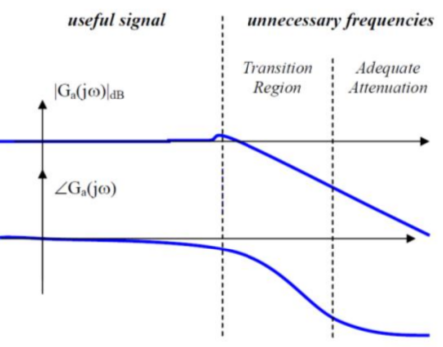
\includegraphics[scale=0.4]{ch4/image3.png}
	\captionof{figure}{ }
	\end{wrapfigure}	
L'idéal serait un filtre gain constant dans la BP et nul en dehors, mais ce n'est pas réalisable 
en pratique. Il faut utiliser un filtre $\mathbb{R}$ possédant une zone de distorsion (la pente 
n'étant pas parfaitement perpendiculaire). Cette zone est un peu floue car elle est polluée par 
le repliement spectral (le "pouvoir filtrant" n'est pas assez important). Cependant, aucune informations 
utiles ne s'y trouve. 

	\subsection{Échantillonnage par une fonction périodique}
	On multiplie (\textbf{pas} une convolution) $x(t)$ par un signal périodique $p(t)$ (pas 
	forcément un train d'impulsions).
	\begin{equation}
	y(t) = x(t)p(t)
	\end{equation}
	Avec $\DS p(t) = \sum_{k=-\infty}^\infty c_ke^{jk\Omega_st}, y(t) =  \sum_{k=-\infty}^\infty 
	c_kx(t)e^{jk\Omega_st}$ on trouve
	\begin{equation}
	Y(\Omega) = \sum_{k=-\infty}^\infty c_k X(\Omega-k\Omega_s)
	\end{equation}
	Le domaine étant continu, $\DS \sum_{k=-\infty}^\infty$ est un nombre infini. On retrouve 
	comme précédemment les spectres décalés (de là vient la règle $1/2T$, \dots). Ici $c_k$ ne 
	vaut plus l'unité mais varie avec la fréquence.
	
	\subsection{Utilisation d'un système à temps discret pour le traitement des signaux à TC}
	On utilise la chaîne suivante, équivalent à un système à TC (si cond. de Shanon OK) 
	\begin{center}
	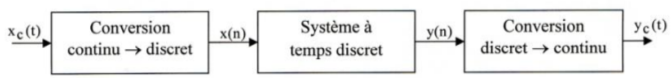
\includegraphics[scale=0.45]{ch4/image4.png}
	\captionof{figure}{ }
	\end{center}
	\begin{enumerate}
	\item \textit{Conversion continu $\rightarrow$ discret}
\begin{center}
			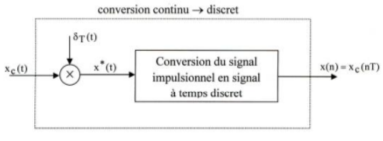
\includegraphics[scale=0.54]{ch4/image8.png}
	\captionof{figure}{ }
\end{center}
	C'est la fameuse multiplication de $x_c(t)$ par $\delta_T(t)$ pour obtenir un signal pulsé. On 
	utilise pour ça un convertisseur analogique-numérique.
	\begin{equation}
	x^*(t) = x_c(t)\sum_{n=-\infty}^\infty \delta(t-nT) = \sum_{n=-\infty}^\infty x_c(nT)
	\delta(t-nT) 
	\end{equation}
	En prenant la transformée de Laplace\footnote{Sachant que $\mathcal{L}(\delta(t))=1$ et le 
	glissement $T \rightarrow e^{-pT}$.} :
	\begin{equation}
	X^*(p) = \sum_{n=-\infty}^\infty x_c(nT)e^{-pnT} = \sum_{n=-\infty}^\infty x_c(nT)e^{-j\Omega nT}
	\end{equation}
	La seconde égalité particularise pour la transformée de Joseph.\\
	
	Pour un signal à temps discret $x(n)$ :
	\begin{equation}
	X(e^{j\omega}) = \sum_{n=-\infty}^\infty x(n)e^{-j\omega n}
	\end{equation}
	Comme $x(n) = x_c(nT)$, on peut écrire (première ligne)
	\begin{equation}
	\begin{array}{ll}
	X(e^{j\omega}) &= \sum_{n=-\infty}^\infty x_c(nT)e^{-j\omega n}\\
	X^*(\Omega) &= \sum_{n=-\infty}^\infty x_c(nT)e^{-j\Omega nT}
	\end{array}
	\end{equation}
	Par identification avec la deuxième ligne, il vient que
	\begin{equation}
	X^*\left(\frac{\omega}{T}\right) = X(e^{j\omega})
	\end{equation}
	La seule différence tren la TF de $x(n)$ (discret) et celle de $x^*(t)$ (impulsionnel) est 
	un changement d'échelle : $\omega = \Omega T$.
	
	\item \textit{Conversion discret $\rightarrow$ continu}
\begin{center}
		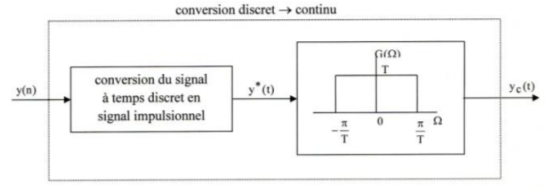
\includegraphics[scale=0.4]{ch4/image7.png}
	\captionof{figure}{ }
\end{center}
	Le signal numérique ayant été transformé, il faut le transmettre en analogique. Si le système à 
	TD possède une réponse en fréquence $F(e^{j\omega})$, la transformée de Fourier de $y(n)$ (discret) 
	sera
	\begin{equation}
	Y(e^{j\omega}) = F(e^{j\omega})X(e^{j\omega})
	\end{equation}
	Passé du monde numérique à pulsé donnera un spectre identique à un facteur près.
	\end{enumerate}
	
	En pratique, on utilise un extrapolateur d'ordre zéro pour reconstruire un signal continu à 
	partir de ses échantillons : un signal analogique doit passer par les points du numérique.
	
		\subsubsection{Reconstitution par un extrapolateur d'ordre zéro}
		Considérons un système à TC de réponse impulsionnelle $h(t)$
		\begin{equation}
		y_c'(t) = y^*(t)*h(t)
		\end{equation}
		où $y^*(t) = \sum_{n=-\infty}^\infty y(n)\delta(t-nT)$ de sorte que l'on ai
		\begin{equation}
		y_c'(t) = \sum_{n=-\infty}^\infty y(n)\delta(t-nT)*h(t) = \sum_{n=-\infty}^\infty y(n)
		h(t-nT)
		\end{equation}
		Il reste à choisir $h(t)$ de sorte à ce que la fonction interpolée passe par les bon 
		points imposés par le numérique. C'est le cas si
		\begin{equation}
		\left\{\begin{array}{ll}
		h(0) &= 1\\
		h(nT) &= 0\qquad \text{ pour } n \neq 0
		\end{array}\right.
		\end{equation}
		Toutes fonctions qui satisfont ça sont des extrapolations. On retrouve bien $y_c'(nT)=y(n)$ 
		: on a une fonction continue $y_c'(t)$ qui prend des valeurs imposées pour $t=nT$.
		
		\exemple{Le filtre passe bas de réponse impulsionnelle $h(t) = \text{sinc}(\pi t/T)$ vérifie 
		ces conditions.}\ 
		
		Pour l'\textbf{extrapolateur d'ordre zéro}, on considère la \textit{fonction escalier}
		\begin{equation}
		h_0(t) = u(t)-u(t-T)
		\end{equation}
		Il s'agit bien d'une fonction continue passant par tous les points. Par calcul de la 
		transformée de Laplace
		\begin{equation}
		h_0(t)\quad\lt\quad \frac{1}{p}-\frac{e^{-pt}}{p}\quad\Longrightarrow\quad
		H_0(\Omega) = \frac{2\sin(\Omega T/2)}{\Omega}e^{-j\Omega T/2}\approx Te^{-j\Omega T/2}\quad 
		\text{ pour }\Omega \ll \frac{2}{T}
		\end{equation}
		
			\begin{wrapfigure}[10]{l}{7cm}
%	\vspace{-5mm}
	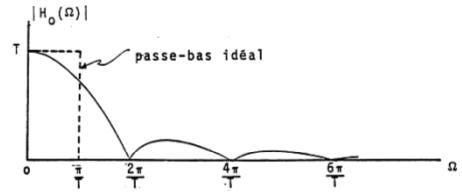
\includegraphics[scale=0.4]{ch4/image5.png}
	\captionof{figure}{ }
	\end{wrapfigure}	
		Cette fonction est assez plate au début puis adopte la forme typique de sinc.
		L'extrapolateur d'ordre zéro va "gommer" les spectres à gauche et à droite de manière 
		partielle : le gain n'est pas constant dans la bande passante qui va forcément causer de 
		légères distorsions dans la bande utile $\DS -\frac{\pi}{T}<\Omega<\frac{\pi}{T}$. De plus, 
		les spectres décallés ne sont pas totalement retirés. Deux solutions 
		\begin{enumerate}
		\item Filtrer pour continuer à gommer.
		\item Compenser par un signal de gain opposé.
		\end{enumerate}
		
	Notons que plutôt que d'interpoler en escalier, on peut utiliser un ordre plus élevée. Pour 
	l'ordre un, on reliera les points par des droits. On utilise généralement une fonction 
	triangle pour $h_1(t)$.
	
	\subsubsection{Chaîne pour le traitement numérique des signaux analogiques}
	\begin{center}
		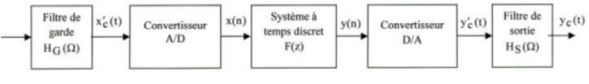
\includegraphics[scale=0.54]{ch4/image6.png}
	\captionof{figure}{ }
	\end{center}
	Un spectre strictement limité n'existe pas : on utilise un filtre anti-repliement pour 
	que l'information dans la bande utile $\DS \left[-\frac{\pi}{T};\frac{\pi}{T}\right]$ ne 
	soit pas altérée, généralement avec un filtre passe bas de $f_c = \pi/T$.\\
	
	La conversion en un signal à TD est réalisée par le convertisseur analogique. Ce signal 
	discret, $x(n)$ est ensuite traité par le système à TD de réponse en fréquence $F$
	\begin{equation}
	Y(e^{j\omega}) = F(e^{j\omega})X(e^{j\omega})
	\end{equation}
	Un signal en escalier $y_c'(t)$ est reconstitué à partir des échantillons de sortie $y(n)$ 
	avec un convertisseur numérique-analogique
	\begin{equation}
	Y_C'(\Omega) = Y^*(\Omega)H_0(\Omega) = Y(e^{j\Omega T})H_0(\Omega)
	\end{equation}
	où $H_0(\Omega)$ est la réponse en fréquence de l'extrapolateur d'ordre zéro. Finalement, 
	un filtre de sortie $H_S(\Omega)$ lisse le signal. Cette démarche (appliquée au slide T41) 
	est une question d'examen.  La fin du chapitre est une série d'exemples.\\

	\begin{center}
		
\includegraphics[scale=0.4]{ch4/image9}
	\captionof{figure}{J'allais pas laisser une page blanche\dots}
\end{center}
	
	
	
	
	
	
	
	
	
	
	
	
	
	
	
	
	
	
	
	
	
	
	
	
	
	
	
	
	
